\section{はじめに}

% \begin{itemize}
%   \item わかるらんどの思想を述べる
%   \item 消去性コンピューティングについて\cite{kurihara2016}
% \end{itemize}

ワイヤレスネットワークや小型計算機の普及による
IoT社会が到来しつある現在,
人々は大量のリアルタイム情報や通知メッセージなどに圧倒されている.
%
多くの情報を人間が理解しやすくするため,
以下のような視覚化手法が利用されている.

\vspace{3mm}

\paragraph*{情報ダッシュボード}

情報ダッシュボード\cite{few}は,
複数のリアルタイム情報をタイル状に並べて表示することによって
多くの情報をわかりやすく視覚化するシステムである.
たとえばWindowsのスタート画面(図\ref{windows})の情報ダッシュボードには
天気予報や株価のようなリアルタイム情報を表示可能である.

\begin{figure}[h]
\centering
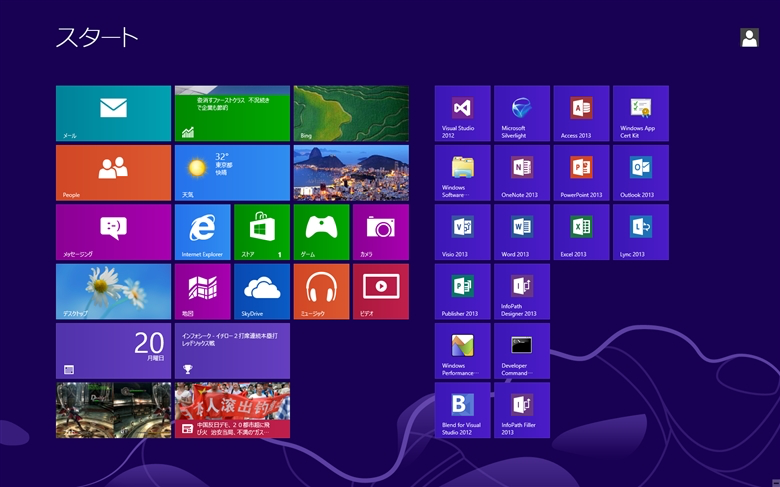
\includegraphics[width=7cm]{images/windows.png}
\caption{Windowsのスタート画面}
\label{windows}
\end{figure}


\vspace{2mm}
\paragraph*{スタンプ}

リアルタイムに流れていくタイムライン表示の中で情報を目立たせたいとき,
近年「スタンプ」と呼ばれるピクトグラムが
利用されることが多くなってきた(図\ref{linestamp}).

スタンプはテキストで記述するのが難しい表現や感情を伝えたり,
テキストを考えて入力するよりも速くて簡単であったりすることから,
近年LINEやFacebookメッセンジャー,オンラインゲームなどで広く利用されている.

\begin{figure}[H]
\centering\fbox{
\includegraphics[width=4cm]{images/linestamp.png}}
\caption{LINEのスタンプの例}
\label{linestamp}
\end{figure}

スタンプ的な表現を投稿可能な情報ダッシュボードを用意し,
その上で
ネット上の情報や
ユーザの感情/気分などを表示すれば,
現在の世界や人々の状況を一目了然に理解する(わかる)ことが可能になるであろう.
%
実世界の状態や人間の状況を情報ダッシュボードにわかりやすく表示し,
かつ誰もが簡単に気分などをスタンプのように投稿して共有できる
「わかるらんど」システムを構築した.



